% !TEX program = pdflatex
% !TEX ext =  --interaction=nonstopmode --enable-etex --enable-write18
% !BIB program = none
%%%==============================================================================
%% Copyright 2024-present by Alceu Frigeri
%%
%% This work may be distributed and/or modified under the conditions of
%%
%% * The [LaTeX Project Public License](http://www.latex-project.org/lppl.txt),
%%   version 1.3c (or later), and/or
%% * The [GNU Affero General Public License](https://www.gnu.org/licenses/agpl-3.0.html),
%%   version 3 (or later)
%%
%% This work has the LPPL maintenance status *maintained*.
%%
%% The Current Maintainer of this work is Alceu Frigeri
%%
%% This is version {1.0} {2024/01/13}
%%
%% The list of files that compose this work can be found in the README.md file at
%% https://ctan.org/pkg/tikzdotncross
%%
%%%==============================================================================
\documentclass[10pt]{article}
\RequirePackage[verbose,a4paper,marginparwidth=27.5mm,top=2.5cm,bottom=1.5cm,hmargin={40mm,20mm},marginparsep=2.5mm,columnsep=10mm,asymmetric]{geometry}
\usepackage{codedescribe}
\RequirePackage[inline]{enumitem}
\SetEnumitemKey{miditemsep}{parsep=0ex,itemsep=0.4ex}

\usepackage[american,siunitx,cuteinductors,smartlabels,arrowmos,EFvoltages,betterproportions]{circuitikz}
\usetikzlibrary{math}
\usepackage{tikzdotncross}
\usepackage{tikzquads}

\RequirePackage{amsmath}
\RequirePackage{amsthm, amssymb, amsfonts}
%\RequirePackage{mathrsfs}
%\RequirePackage{mathtools}
%\RequirePackage{empheq}
%\RequirePackage{cases}
%\RequirePackage{extarrows}
%\RequirePackage{mathfixs}

\RequirePackage[hidelinks,hypertexnames=false]{hyperref}



\NewDocumentCommand{\pinanchors}{mm}{ \path \foreach \n/\a/\d in {#2} { (#1.\n) \pincoord(\n,blue,\a,\d)}; }
\NewDocumentCommand{\pingeoanchors}{m}{ \pinanchors{#1}{%
    north/90/4, north east/55/4, east/0/4,%
    south east/-55/4,%
    south/-90/4, south west/-100/4, west/180/4, north west/100/4,%
    center/-165/17}
}


\NewDocumentCommand{\pinquadanchors}{m}{%
  \pinanchors{#1}{%
      1+/135/4, 1-/225/4, 2+/45/4, 2-/-45/4, inner 1+/-45/2, inner 1-/45/2, inner 2+/225/2, inner 2-/135/2
  }
}

\NewDocumentCommand{\pinblackboxanchors}{m}{%
  \pinanchors{#1}{%
      1+/135/4, 1-/225/4, inner 1+/-45/2, inner 1-/45/2
  }
}

\NewDocumentCommand{\pinquadtextanchors}{m}{%
   \pinanchors{#1}{%
      bottom left/225/4, bottom center/-90/4, bottom right/-45/4, 
      inner bottom left/225/4, inner bottom center/90/2, inner bottom right/-45/4,
      top left/135/4, top center/90/4, top right/45/4, 
      inner top left/135/4, inner top center/-90/2, inner top right/45/4
   } 
}

\begin{document}
\tstitle{
  author={Alceu Frigeri\footnote{\tsverb{https://github.com/alceu-frigeri/tikzquads}}},
  date={\tsdate},
  title={The tikzquads Package\break An Extension to CircuiTi\emph{k}Z\break Version \PkgInfo{tikzquads}{version}}
  }
  

\begin{typesetabstract}
 
This package defines a few extra shapes (single / dual port boxes) designed to be used together with the \tsobj[pkg]{CircuiTikZ} package.
\end{typesetabstract}

\tableofcontents

\section{Introduction}
In standard text books, both for Circuits Theory and Electronics, quite frequently, in the process of modelling sub-circuits, one ends representing them  either:
\begin{itemize}
  \item as a single port \emph{black box}, or
  \item as a dual port \emph{black box}
\end{itemize}

This package defines a few, parameterized shapes for each case:
\begin{itemize}
  \item for single port \emph{black boxes}:
  \begin{itemize}
    \item Black Box
    \item Thevenin
    \item Norton
  \end{itemize}
  \item for dual port \emph{black boxes}:
  \begin{itemize}
    \item Quad
    \item Quad Z
    \item Quad Y
    \item Quad G
    \item Quad H
  \end{itemize}
Lastly, this package also defines a \emph{Pseudo-Graph load line} shape, for those moments where a true graph, \tsobj[pkg]{pgfplots}, isn't needed.
\end{itemize}
 
 \subsection{CircuiTi\emph{k}Z}
 Unfortunately, some implementation details of these shapes don't follow the code structure  adopted by \tsobj[pkg]{CircuiTikZ}, and some significant part of this package's code would have to be re-written if it were to be integrated directly in \tsobj[pkg]{CircuiTikZ}, and that's the main reason this is, for the time being, a separate package. After all, even though this doesn't follows \tsobj[pkg]{CircuiTikZ} code scheme, it does work nicely with it, as is.
 
\section{Auxiliary Shapes and Basic Keys}
Those shapes are not intended for end users.

\subsection{Auxiliary shapes}\label{auxiliarynodes}
A set of auxiliary shapes are defined, but not meant to be used otherwise, though their anchors might be relevant:

\begin{center}
\resizebox{0.8\textwidth}{!}{
\begin{tikzpicture}
  \draw (0,0) node[QuadKeys,generic,H Res shape](N){};
  \pingeoanchors{N}
  \draw (4,0) node[QuadKeys,H Res shape](N){};
  \pingeoanchors{N}
  \draw (8,0) node[QuadKeys,generic,V Res shape](N){};
  \pingeoanchors{N}
  \draw (12,0) node[QuadKeys,V Res shape](N){};
  \pingeoanchors{N}

  \draw (0,-2) node[QuadKeys,round sources,IsourceDOWN shape](N){};
  \pingeoanchors{N}
  \draw (4,-2) node[QuadKeys,IsourceDOWN shape](N){};
  \pingeoanchors{N}
  \draw (8,-2) node[QuadKeys,round sources,IsourceUP shape](N){};
  \pingeoanchors{N}
  \draw (12,-2) node[QuadKeys,IsourceUP shape](N){};
  \pingeoanchors{N}

  \draw (0,-4) node[QuadKeys,round sources,Vsource shape](N){};
  \pingeoanchors{N}
  \draw (4,-4) node[QuadKeys,Vsource shape](N){};
  \pingeoanchors{N}
  
\end{tikzpicture}}
\end{center}

\begin{tsremark}
The point being that, regardless of the sub-shape orientation, the intuitive geographical coordinates applies.
\end{tsremark}


        
\subsection{General Keys}\label{generalkeys}
These are the keys to fine tuning a shape:
\begin{describelist*}[30mm]{keys}
  \describe {outer sep}  {Text outer separation, initial value: 1.5pt}
  \describe {inner sep}  {Text inner separation, initial value: 1pt}
  \describe {thickness} {Components thickness (relative to the drawing thickness), initial value: 2}
  \describe {tip len} {tip len (current source). initial value: 4pt}
  \describe {tip type} {possible values: \tsobj[keys]{triangle,bezier}. initial value: \tsobj[keys]{triangle}}
  \describe {minussign len}  {Minus sign len (voltage source). initial value: \tsobj{\pgf@circ@Rlen/14}}
  \describe {plussign len}  {Plus sign len (voltage source). initial value: \tsobj{1.1\pgf@circ@Rlen/14}}
  \describe {source radius} {The base radius. initial value: \tsobj{0.3\pgf@circ@Rlen}}
  \describe {round sources} {Sources will be round ones}
  \describe {control sources} {Sources will be control/diamond ones}
  \describe {generic, european} {Impedances will be generic rectangles}
  \describe {zigzag, american} {Impedances will be draw as zigzags}
\end{describelist*}


%  \describe {name}  {\tsmeta{node-name}, when using a to[\,] path.}


\section{Z, Y, G, H Quadripoles}\label{quadanchors}
A set of configurable Quadripoles is defined, whereas quadripoles parameters (for instance $Z_{11}$, $Z_{12}$, $Z_{21}$ and $Z_{22}$) are \tsobj[marg]{key-value} parameters.
\subsection{The Base Quadripole Shape}
The base shape just draws a base box and sets some connection anchors: $1+$, $1-$, $inner\ 1+$, $inner\ 1-$, $2+$, $2-$, $inner\ 2+$ and $inner\ 2-$, besides the geographic ones:

%,label bottom left={T1},label bottom center={T2},label bottom right={T3}

\begin{center}%
  \resizebox{0.8\textwidth}{!}{%
    \begin{tikzpicture}
      \draw (0,0) node[Quad](Qa){text};
      \pingeoanchors{Qa}
      \draw (Qa.2+) ++(2,0) node[Quad,anchor=1+](Qb){text};
      \pinquadanchors{Qb}
    \end{tikzpicture}
  }
\end{center}

And also a set of (meant for) \emph{text} anchors:

\begin{center}
  \resizebox{0.4\textwidth}{!}{
    \begin{tikzpicture}
      \draw (0,0)  node[Quad](Qc){text};
      \pinquadtextanchors{Qc}
    \end{tikzpicture}
  }
\end{center}

        

\subsubsection{Base Keys}\label{quadkeys}
These applies to all Quad shapes:
\begin{describelist*}[30mm]{keys}
  \describe {base width}  {The 'box' width}
  \describe {half base width}  {Ditto, half width. Initial value:\tsobj{2\pgf@circ@Rlen}.}
  \describe {base height}  {The distance between \tsobj[keys]{1+,1-}. The 'box' full height is equal to 2*(\tsobj[keys]{half base height} + \tsobj[keys]{height ext} + \tsobj[keys]{height ext+}).}
  \describe {half base height} {Ditto, half height. Initial value:\tsobj{\pgf@circ@Rlen/7} }
  \describe {height ext}{Initial value:\tsobj{2\pgf@circ@Rlen/7}}
  \describe {height ext+}{Initial value:0}  
  \describe {inner ext} {distance between the 'box' and \tsobj{inner 1+/1-/2+/2-}. initial value: \tsobj{\pgf@circ@Rlen/7}}
  \describe {outer ext} {distance between the 'box' and \tsobj{1+/1-/2+/2-}. initial value: \tsobj{5\pgf@circ@Rlen/14}}
  \describe {inner marks}  {If set, the inner anchors will be marked.}
  \describe {outer marks}  {If set, the outer anchors will be marked.}
  \describe {invert} {The shape will be inverted, more or less like 'x scale=-1'.}
  \describe {alt, opt} {Case a Voltage source is zero, a series impedance will be draw vertically.}
  \describe {outer x fit to} {For any Quad, this is the same as \tsobj[key]{outer x fit to*}.}
  \describe {outer x fit to*} {\tsobj[keys]{outer x fit*=}\tsargs[marg]{CoordA,CoordB}. The width will be set so that \tsobj[meta]{1+,2+} (or \tsobj[meta]{1-,2-}, depending on the used anchor) \textbf{will fit} \tsobj[meta]{CoordA,CoordB}. This might result in a shape rotation.}
  \describe {outer x fit to!} {\tsobj[keys]{outer x fit!=}\tsargs[marg]{CoordA,CoordB}. The width will be set so that the distance between \tsobj[meta]{1+,2+} (or \tsobj[meta]{1-,2-}, depending on the used anchor) will be the same as \tsobj[meta]{CoordA,CoordB}. This will never result in a shape rotation.} 
  \describe {inner x fit to} {For any Quad, this is the same as \tsobj[key]{inner x fit to*}.}
  \describe {inner x fit to*} {\tsobj[keys]{inner x fit*=}\tsargs[marg]{CoordA,CoordB}. The width will be set so that \tsobj[meta]{inner 1+,inner 2+} (or \tsobj[meta]{inner 1-,inner 2-}, depending on the used anchor) \textbf{will fit} \tsobj[meta]{CoordA,CoordB}. This might result in a shape rotation.} 
  \describe {inner x fit to!} {\tsobj[keys]{inner x fit!=}\tsargs[marg]{CoordA,CoordB}. The width will be set so that the distance between \tsobj[meta]{inner 1+,inner 2+} (or \tsobj[meta]{inner 1-,inner 2-}, depending on the used anchor) will be the same as \tsobj[meta]{CoordA,CoordB}. This will never result in a shape rotation.}
  \describe {y fit to} {For any Quad, this is the same as \tsobj[key]{y fit to!}.}
  \describe {y fit to*} {\tsobj[keys]{y fit*=}\tsargs[marg]{CoordA,CoordB}.   The height will be set so that \tsobj[keys]{1+,1-} \textbf{will fit} \tsobj[keys]{CoordA,CoordB}. This might result in a shape rotation} 
  \describe {y fit to!} {\tsobj[keys]{y fit!=}\tsargs[marg]{CoordA,CoordB}. The height will be set so that the distance between \tsobj[meta]{1+,1-} will be equal to the distance between \tsobj[marg]{CoordA,CoordB}. This will never result in a shape rotation.}
%  
%  \describe {outer x fit to} {\tsobj[keys]{outer x fit=}\tsargs[marg]{CoordA,CoordB}. The width will be set so that \tsobj[meta]{1+,2+} (or \tsobj[meta]{1-,2-}, depending on the used anchor) will fit \tsobj[meta]{CoordA,CoordB}}
%  \describe {outer x fit to*} {Same as \tsobj[key]{outer x fit to}, might result in a rotation.} 
%  \describe {outer x fit to!} {Same as \tsobj[key]{outer x fit to}, but will never result in a rotation.} 
%  \describe {inner x fit to} {\tsobj[keys]{inner x fit=}\tsargs[marg]{CoordA,CoordB}. The width will be set so that \tsobj[meta]{inner 1+,inner 2+} (or \tsobj[meta]{inner 1-,inner 2-}, depending on the used anchor) will fit \tsobj[meta]{CoordA,CoordB}}
%  \describe {inner x fit to*} {Same as \tsobj[key]{inner x fit to}, might result in a rotation.} 
%  \describe {inner x fit to!} {Same as \tsobj[key]{inner x fit to}, but will never result in a rotation.} 
%  \describe {y fit to} {\tsobj[keys]{y fit=}\tsargs[marg]{CoordA,CoordB}. The distance between, lets say \tsobj[keys]{1+,1-} will be made equal to the distance between \tsobj[keys]{CoordA,CoordB}.}
%  \describe {y fit to*} {Same as \tsobj[key]{y fit to}, might result in a rotation.} 
%  \describe {y fit to!} {Same as \tsobj[key]{y fit to}, but will never result in a rotation.} 
  \describe{label top left}{It will place a label at the top left anchor}
  \describe{label top center}{It will place a label at the top center anchor}
  \describe{label top right}{It will place a label at the top right anchor}
  \describe{label inner top left}{It will place a label at the inner top left anchor}
  \describe{label inner top center}{It will place a label at the inner top center anchor}
  \describe{label inner top right}{It will place a label at the inner top right anchor}
  \describe{label bottom left}{It will place a label at the bottom left anchor}
  \describe{label bottom center}{It will place a label at the bottom center anchor}
  \describe{label bottom right}{It will place a label at the bottom right anchor}
  \describe{label inner bottom left}{It will place a label at the inner bottom left anchor}
  \describe{label inner bottom center}{It will place a label at the inner bottom center anchor}
  \describe{label inner bottom right}{It will place a label at the inner bottom right anchor}
\end{describelist*}
%\begin{tsremark}
%For Quadripoles, \tsobj[keys]{outer x fit, inner x fit} might result in a shape rotation. \tsobj[keys]{y fit} never will result in a rotation.
%\end{tsremark}
%\begin{tsremark}
%Those keys can be used with all the following components: \tsobj[meta]{Quad,Quad Z,Quad Y,Quad G,Quad H,ToQuad,ToQuad Z,ToQuad Y,ToQuad G,ToQuad H,Black Box,Thevenin,Norton,ToBlack Box,ToThevenin,ToNorton}.
%\end{tsremark}


A small example of the \emph{fit to} keys:
\begin{codestore}[QuadKeysA]
\begin{tikzpicture}
\draw (0,0)  \pincoord(A,blue,225) ++(4,0)  \pincoord(B,blue,-45) ++(2,2)  \pincoord(C) ;

\draw (A) node[Quad,anchor=1+,outer x fit to={A}{B}](Qa){\footnotesize$Qa$};
\draw (B) node[Quad,anchor=1+,outer x fit to={B}{C},I1=$I_a$,V2=$V_b$](Qb){\footnotesize$Qb$};

\draw (Qb.2-) -- ++(2,0)  \pincoord(D) ++(1,-2) \pincoord(E);

\draw (D) node[Black Box,anchor=1+,y fit to={D}{E}](Ba){\footnotesize$Ba$};

\draw (Qa.1-) ++(0,-1);
\end{tikzpicture}
\end{codestore}

\tsdemo*[codeprefix={},resultprefix={},emph={draw,node},basicstyle={\scriptsize\ttfamily},numbers=left]{QuadKeysA}



% show anchors of a node component:
% optional: options of the circuitikz environment
% mandatory  node spec, node text
% optional between (): anchor specification list
\NewDocumentCommand{\showsubanchors}{O{} m m m d()}
{
       \begin{circuitikz}[#1]
              \draw   (0,0) node[#2](N){#3};
            \IfValueT{#5}{%
                \foreach \sn in {#4} {%
                  \foreach \n/\a/\d in {#5} {%
                   \path (N-\sn.\n) \showcoord(\n)<\a:\d>;
                  }
                }
            }
            ;\par
        \end{circuitikz}%
}

\subsection{Quad}
\begin{codestore}[QuadDef]
% Node use
node[Quad]{}

% To path use
(A) to[ToQuad]  (B)
\end{codestore}

\tscode*[emph={draw,node},emph2={x,y,fit,to,outer,inner,node},emph3={Quad,ToQuad,Black,ToBlack,Box,Thevenin,ToThevenin,Norton,ToNorton},basicstyle={\scriptsize\ttfamily},numbers=left,codeprefix={}]{QuadDef}

This is just the base shape, to be used in cases whereas one just want to emphasises part of a circuit (using, for instance, the \tsobj[key]{inner x fit to} key, or just mark a two port black box.
\begin{tsremark}
There is also a \tsobj[key]{ToQuad} to be used in a \tsobj[key]{to[ ]} path, in which case the key \tsobj[key]{outer x fit to} style will be triggered with the starting and ending points of the \tsobj[key]{to[ ]} path.
\end{tsremark}

\begin{center}%
  \resizebox{0.8\textwidth}{!}{%
    \begin{tikzpicture}
      \draw (0,0) node[Quad](Qa){text};
      \pingeoanchors{Qa}
      \draw (Qa.2+) ++(2,0) node[Quad,anchor=1+](Qb){text};
      \pinquadanchors{Qb}

      \draw (Qa.2-) ++(1,-1.5)  node[Quad,anchor=north](Qc){text};
      \pinquadtextanchors{Qc}
    \end{tikzpicture}
  }
\end{center}

\subsubsection{Quad Keys}
\begin{describelist*}{keys}
  \describe {name}  {\tsmeta{node-name}, when using a to[\,] path.}
  \describe{I1}{Initial value:\tsverb{$I_1$}}
  \describe{I2}{Initial value:\tsverb{$I_2$}}
  \describe{V1}{Initial value:\tsverb{$V_1$}}
  \describe{V2}{Initial value:\tsverb{$V_2$}}
\end{describelist*}


\subsubsection{Examples of \emph{fit to} use}
Squeezing a Quadripole between two parts of a circuit (nodes C and D):

\begin{codestore}[QuadfitA]
\begin{center}
  \resizebox{0.5\textwidth}{!}{
    \begin{tikzpicture}
      \draw (0,0) \pincoord(ref) to[R=R1] ++(0,2)  \pincoord(A)  to[R=R2] ++(0,2) \pincoord(B)
      -- ++(2,0)  \pincoord(C,red,225) (C |- ref)  \pincoord(C1,blue,135) -- (ref);
      \draw (C) ++(7,0)  \pincoord(D,red) -- ++(0.5,0) to[R=R3] ++(0,-3) -- ++(2,0) to[R=R4] ++(0,3) -- ++(0.5,0)   \pincoord(E);
      \draw (C) node[Quad,anchor=1+,y fit to={C}{C1},outer x fit to={C}{D}]{};
    \end{tikzpicture}
  }
\end{center}
\end{codestore}

\tsdemo*[codeprefix={},resultprefix={},emph={draw,node},emph2={x,y,fit,to,outer,inner,node},emph3={Quad,Black,Box},basicstyle={\scriptsize\ttfamily},numbers=left]{QuadfitA}

~

Fitting some circuit inside the Quadripole (nodes C and E):
\begin{codestore}[QuadfitB]
\resizebox{0.4\textwidth}{!}{
\begin{tikzpicture}
  \draw (0,0) \pincoord(ref) to[R=R1] ++(0,2) \pincoord(A)  to[R=R2] ++(0,2) \pincoord(B)
  -- ++(2,0) \pincoord(C,red) (C |- ref) \pincoord(C1) -- (ref);
  \draw (C) ++(7,0)  \pincoord(D) -- ++(0.5,0) to[R=R3] ++(0,-3) -- ++(2,0) to[R=R4] ++(0,3) -- ++(0.5,0)  \pincoord(E,red);
  \draw (C) node[Quad,anchor=inner 1+,y fit to={C}{C1},inner x fit to={C}{E}]{};
\end{tikzpicture}}
\end{codestore}

\tsdemo*[codeprefix={},resultprefix={},emph={draw,node},emph2={x,y,fit,to,outer,inner,node},emph3={Quad,Black,Box},basicstyle={\scriptsize\ttfamily},numbers=left]{QuadfitB}



\subsection{Quad Z}
\begin{codestore}[QuadZDef]
% Node use
node[Quad Z]{}

% To path use
(A) to[ToQuad Z]  (B)
\end{codestore}

\tscode*[emph={draw,node},emph2={x,y,fit,to,outer,inner,node},emph3={Quad,ToQuad,Black,ToBlack,Box,Thevenin,ToThevenin,Norton,ToNorton},basicstyle={\scriptsize\ttfamily},numbers=left,codeprefix={}]{QuadZDef}

This shape, besides the base anchors (see \ref{quadanchors}) it has 4 internal nodes: \tsobj[key]{<node>-Z11,<node>-Z12,<node>-Z21,<node>-Z22}  and each of those sub-nodes has geographic anchors as defined at \ref{auxiliarynodes}.
\begin{tsremark}
There is also a \tsobj[key]{ToQuad Z} to be used in a \tsobj[key]{to[ ]} path, in which case the key \tsobj[key]{outer x fit to} style will be triggered with the starting and ending points of the \tsobj[key]{to[ ]} path.
\end{tsremark}

\begin{center}%
  \resizebox{0.8\textwidth}{!}{%
    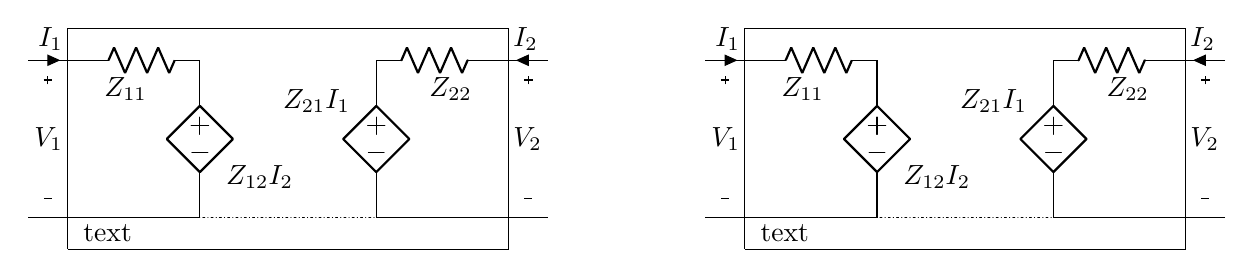
\begin{tikzpicture}
      \draw (0,0) node[Quad Z](Qa){text};
      \pingeoanchors{Qa}
      \draw (Qa.2+) ++(2,0) node[Quad Z,anchor=1+](Qb){text};
      \pinquadanchors{Qb}
    \end{tikzpicture}
  }
\end{center}
\begin{center}%
  \resizebox{0.4\textwidth}{!}{%
    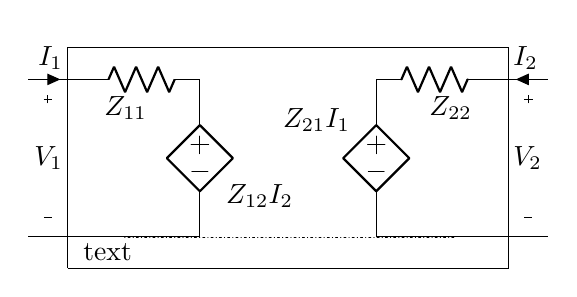
\begin{tikzpicture}
      \draw (0,0)  node[Quad Z,anchor=north](Qc){text};
      \pinquadtextanchors{Qc}
    \end{tikzpicture}
  }
\end{center}

\subsubsection{Quad Z keys}
\begin{describelist*}[30mm]{keys}
  \describe {name}  {\tsmeta{node-name}, when using a to[\,] path.}
  \describe{I1}{Initial value:\tsverb{$I_1$}}
  \describe{I2}{Initial value:\tsverb{$I_2$}}
  \describe{V1}{Initial value:\tsverb{$V_1$}}
  \describe{V2}{Initial value:\tsverb{$V_2$}}
  \describe{Z11}{Initial value:\tsverb{$Z_{11}$}}
  \describe{Z12}{Initial value:\tsverb{$Z_{12}$}}
  \describe{Z21}{Initial value:\tsverb{$Z_{21}$}}
  \describe{Z22}{Initial value:\tsverb{$Z_{22}$}}
  \describe{Z11 label pos}{changes the label position. Defaults to: \tsobj[verb]{{south west}{top left}}}
  \describe{Z12 label pos}{changes the label position. Defaults to: \tsobj[verb]{{south east}{top left}}}
  \describe{Z21 label pos}{changes the label position. Defaults to: \tsobj[verb]{{north west}{bottom right}}}
  \describe{Z22 label pos}{changes the label position. Defaults to: \tsobj[verb]{{south east}{top right}}}
\end{describelist*}
\begin{tsremark}
The label pos keys expects two anchor names (... label pos=\tsargs[marg]{anchor A,anchor B}). The first anchors refers the sub-shape node and the second anchor is the text one.
\end{tsremark}



\subsection{Quad Y}
\begin{codestore}[QuadYDef]
% Node use
node[Quad Y]{}

% To path use
(A) to[ToQuad Y]  (B)
\end{codestore}

\tscode*[emph={draw,node},emph2={x,y,fit,to,outer,inner,node},emph3={Quad,ToQuad,Black,ToBlack,Box,Thevenin,ToThevenin,Norton,ToNorton},basicstyle={\scriptsize\ttfamily},numbers=left,codeprefix={}]{QuadYDef}
This shape, besides the base anchors (see \ref{quadanchors}) it has 4 internal nodes: \tsobj[key]{<node>-Y11,<node>-Y12,<node>-Y21,<node>-Y22}  and each of those sub-nodes has geographic anchors as defined at \ref{auxiliarynodes}.
\begin{tsremark}
There is also a \tsobj[key]{ToQuad Y} to be used in a \tsobj[key]{to[ ]} path, in which case the key \tsobj[key]{outer x fit to} style will be triggered with the starting and ending points of the \tsobj[key]{to[ ]} path.
\end{tsremark}

\begin{center}%
  \resizebox{0.8\textwidth}{!}{%
    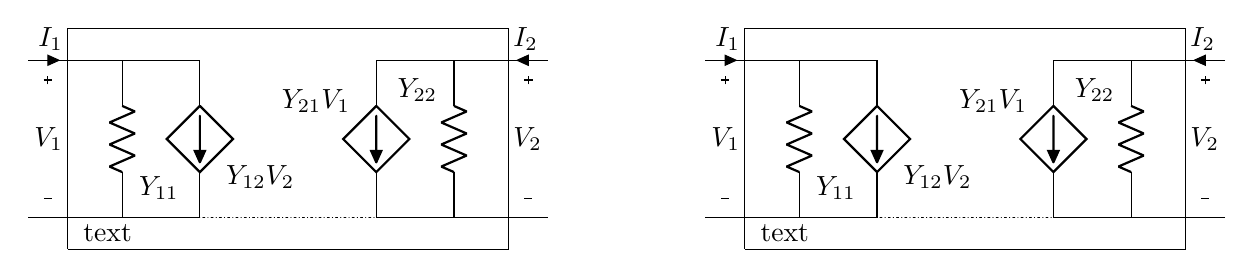
\begin{tikzpicture}
      \draw (0,0) node[Quad Y](Qa){text};
      \pingeoanchors{Qa}
      \draw (Qa.2+) ++(2,0) node[Quad Y,anchor=1+](Qb){text};
      \pinquadanchors{Qb}
    \end{tikzpicture}
  }
\end{center}
\begin{center}%
  \resizebox{0.4\textwidth}{!}{%
    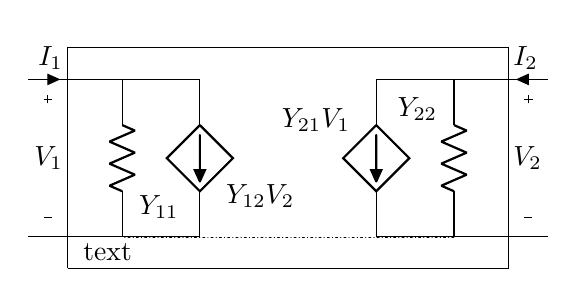
\begin{tikzpicture}
      \draw (0,0)  node[Quad Y,anchor=north](Qc){text};
      \pinquadtextanchors{Qc}
    \end{tikzpicture}
  }
\end{center}

\subsubsection{Quad Y keys}
\begin{describelist*}[30mm]{keys}
  \describe {name}  {\tsmeta{node-name}, when using a to[\,] path.}
  \describe{I1}{Initial value:\tsverb{$I_1$}}
  \describe{I2}{Initial value:\tsverb{$I_2$}}
  \describe{V1}{Initial value:\tsverb{$V_1$}}
  \describe{V2}{Initial value:\tsverb{$V_2$}}
  \describe{Y11}{Initial value:\tsverb{$Y_{11}$}}
  \describe{Y12}{Initial value:\tsverb{$Y_{12}$}}
  \describe{Y21}{Initial value:\tsverb{$Y_{21}$}}
  \describe{Y22}{Initial value:\tsverb{$Y_{22}$}}
  \describe{Y11 label pos}{changes the label position. Defaults to: \tsobj[verb]{{south west}{top left}}}
  \describe{Y12 label pos}{changes the label position. Defaults to: \tsobj[verb]{{south east}{top left}}}
  \describe{Y21 label pos}{changes the label position. Defaults to: \tsobj[verb]{{north west}{bottom right}}}
  \describe{Y22 label pos}{changes the label position. Defaults to: \tsobj[verb]{{north west}{bottom right}}}
\end{describelist*}
\begin{tsremark}
The label pos keys expects two anchor names (... label pos=\tsargs[marg]{anchor A,anchor B}). The first anchors refers the sub-shape node and the second anchor is the text one.
\end{tsremark}

\subsection{Quad G}
\begin{codestore}[QuadGDef]
% Node use
node[Quad G]{}

% To path use
(A) to[ToQuad G]  (B)
\end{codestore}

\tscode*[emph={draw,node},emph2={x,y,fit,to,outer,inner,node},emph3={Quad,ToQuad,Black,ToBlack,Box,Thevenin,ToThevenin,Norton,ToNorton},basicstyle={\scriptsize\ttfamily},numbers=left,codeprefix={}]{QuadGDef}

This shape, besides the base anchors (see \ref{quadanchors}) it has 4 internal nodes: \tsobj[key]{<node>-G11,<node>-G12,<node>-G21,<node>-G22}  and each of those sub-nodes has geographic anchors as defined at \ref{auxiliarynodes}.
\begin{tsremark}
There is also a \tsobj[key]{ToQuad G} to be used in a \tsobj[key]{to[ ]} path, in which case the key \tsobj[key]{outer x fit to} style will be triggered with the starting and ending points of the \tsobj[key]{to[ ]} path.
\end{tsremark}

\begin{center}%
  \resizebox{0.8\textwidth}{!}{%
    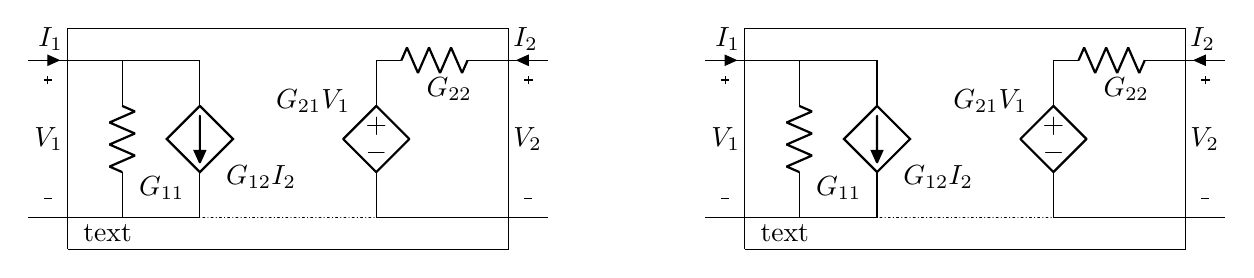
\begin{tikzpicture}
      \draw (0,0) node[Quad G](Qa){text};
      \pingeoanchors{Qa}
      \draw (Qa.2+) ++(2,0) node[Quad G,anchor=1+](Qb){text};
      \pinquadanchors{Qb}
    \end{tikzpicture}
  }
\end{center}
\begin{center}%
  \resizebox{0.4\textwidth}{!}{%
    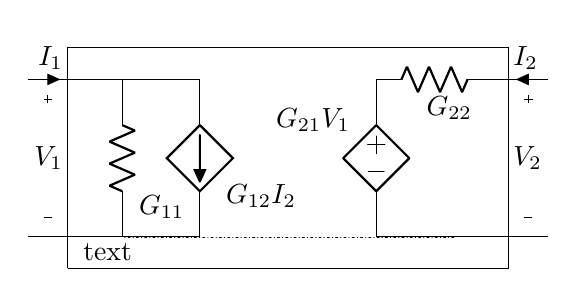
\begin{tikzpicture}
      \draw (0,0)  node[Quad G,anchor=north](Qc){text};
      \pinquadtextanchors{Qc}
    \end{tikzpicture}
  }
\end{center}


\subsubsection{Quad G keys}
\begin{describelist*}[30mm]{keys}
  \describe {name}  {\tsmeta{node-name}, when using a to[\,] path.}
  \describe{I1}{Initial value:\tsverb{$I_1$}}
  \describe{I2}{Initial value:\tsverb{$I_2$}}
  \describe{V1}{Initial value:\tsverb{$V_1$}}
  \describe{V2}{Initial value:\tsverb{$V_2$}}
  \describe{G11}{Initial value:\tsverb{$G_{11}$}}
  \describe{G12}{Initial value:\tsverb{$G_{12}$}}
  \describe{G21}{Initial value:\tsverb{$G_{21}$}}
  \describe{G22}{Initial value:\tsverb{$G_{22}$}}
  \describe{G11 label pos}{changes the label position. Defaults to: \tsobj[verb]{{south west}{top left}}}
  \describe{G12 label pos}{changes the label position. Defaults to: \tsobj[verb]{{south east}{top left}}}
  \describe{G21 label pos}{changes the label position. Defaults to: \tsobj[verb]{{north west}{bottom right}}}
  \describe{G22 label pos}{changes the label position. Defaults to: \tsobj[verb]{{south east}{top right}}}  
\end{describelist*}
\begin{tsremark}
The label pos keys expects two anchor names (... label pos=\tsargs[marg]{anchor A,anchor B}). The first anchors refers the sub-shape node and the second anchor is the text one.
\end{tsremark}

\subsection{Quad H}
\begin{codestore}[QuadHDef]
% Node use
node[Quad H]{}

% To path use
(A) to[ToQuad H]  (B)
\end{codestore}

\tscode*[emph={draw,node},emph2={x,y,fit,to,outer,inner,node},emph3={Quad,ToQuad,Black,ToBlack,Box,Thevenin,ToThevenin,Norton,ToNorton},basicstyle={\scriptsize\ttfamily},numbers=left,codeprefix={}]{QuadHDef}

This shape, besides the base anchors (see \ref{quadanchors}) it has 4 internal nodes: \tsobj[key]{<node>-H11,<node>-H12,<node>-H21,<node>-H22}  and each of those sub-nodes has geographic anchors as defined at \ref{auxiliarynodes}.
\begin{tsremark}
There is also a \tsobj[key]{ToQuad H} to be used in a \tsobj[key]{to[ ]} path, in which case the key \tsobj[key]{outer x fit to} style will be triggered with the starting and ending points of the \tsobj[key]{to[ ]} path.
\end{tsremark}

\begin{center}%
  \resizebox{0.8\textwidth}{!}{%
    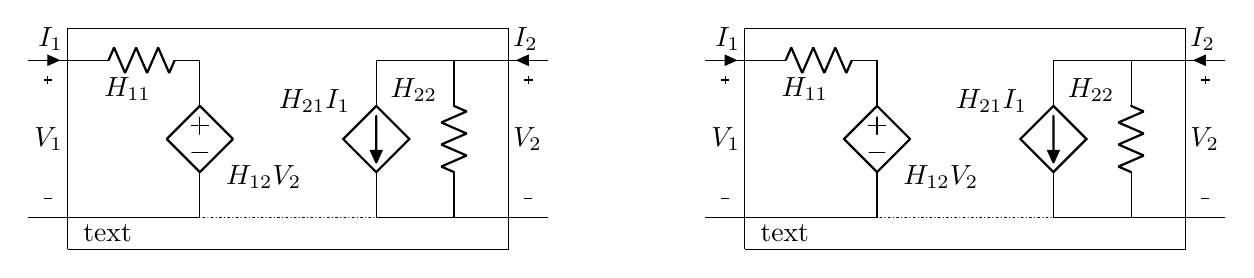
\begin{tikzpicture}
      \draw (0,0) node[Quad H](Qa){text};
      \pingeoanchors{Qa}
      \draw (Qa.2+) ++(2,0) node[Quad H,anchor=1+](Qb){text};
      \pinquadanchors{Qb}
    \end{tikzpicture}
  }
\end{center}
\begin{center}%
  \resizebox{0.4\textwidth}{!}{%
    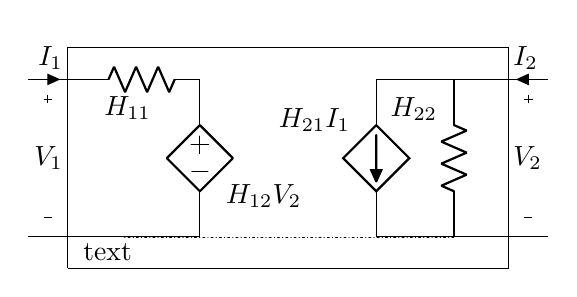
\begin{tikzpicture}
      \draw (0,0)  node[Quad H,anchor=north](Qc){text};
      \pinquadtextanchors{Qc}
    \end{tikzpicture}
  }
\end{center}



\subsubsection{Quad H keys}
\begin{describelist*}[30mm]{keys}
  \describe {name}  {\tsmeta{node-name}, when using a to[\,] path.}
  \describe{I1}{Initial value:\tsverb{$I_1$}}
  \describe{I2}{Initial value:\tsverb{$I_2$}}
  \describe{V1}{Initial value:\tsverb{$V_1$}}
  \describe{V2}{Initial value:\tsverb{$V_2$}}
  \describe{H11}{Initial value:\tsverb{$H_{11}$}}
  \describe{H12}{Initial value:\tsverb{$H_{12}$}}
  \describe{H21}{Initial value:\tsverb{$H_{21}$}}
  \describe{H22}{Initial value:\tsverb{$H_{22}$}}
  \describe{H11 label pos}{changes the label position. Defaults to: \tsobj[verb]{{south west}{top left}}}
  \describe{H12 label pos}{changes the label position. Defaults to: \tsobj[verb]{{south east}{top left}}} 
  \describe{H21 label pos}{changes the label position. Defaults to: \tsobj[verb]{{north west}{bottom right}}}
  \describe{H22 label pos}{changes the label position. Defaults to: \tsobj[verb]{{north west}{bottom right}}}
\end{describelist*}

\begin{tsremark}
The label pos keys expects two anchor names (... label pos=\tsargs[marg]{anchor A,anchor B}). The first anchors refers the sub-shape node and the second anchor is the text one.
\end{tsremark}

~

\section{Thevenin, Norton single port boxes}


\subsection{The Base Black Box Shape}\label{BBanchors}

The base shape just draws a base box and sets some connection anchors: $1+$, $1-$, $inner\ 1+$, $inner\ 1-$, besides the geographic and text ones:


\begin{center}%
  \resizebox{0.8\textwidth}{!}{%
    \begin{tikzpicture}
      \draw (0,0) node[Black Box](Qa){text};
      \pingeoanchors{Qa}
      \draw (Qa.east) ++(2,0) node[Black Box,anchor=west](Qb){text};
      \pinblackboxanchors{Qb}
      \draw (Qb.east) ++(2,0) node[Black Box,anchor=west](Qc){text};
      \pinquadtextanchors{Qc}
    \end{tikzpicture}
  }
\end{center}

        
~   

\subsubsection{Base Keys}\label{BBkeys}

These applies to all \emph{Black Box} shapes:

\begin{describelist*}[30mm]{keys}
  \describe {base width}  {The 'box' width}
  \describe {half base width}  {Ditto, half width. Initial value:\tsobj{2\pgf@circ@Rlen}.}
  \describe {base height}  {The distance between \tsobj[keys]{1+,1-}. The 'box' full height is equal to 2*(\tsobj[keys]{half base height} + \tsobj[keys]{height ext} + \tsobj[keys]{height ext+}).}
  \describe {half base height} {Ditto, half height. Initial value:\tsobj{\pgf@circ@Rlen/7} }
  \describe {height ext}{Initial value:\tsobj{2\pgf@circ@Rlen/7}}
  \describe {height ext+}{Initial value:0}  
  \describe {inner ext} {distance between the 'box' and \tsobj{inner 1+/1-/2+/2-}. initial value: \tsobj{\pgf@circ@Rlen/7}}
  \describe {outer ext} {distance between the 'box' and \tsobj{1+/1-/2+/2-}. initial value: \tsobj{5\pgf@circ@Rlen/14}}
  \describe {inner marks}  {If set, the inner anchors will be marked.}
  \describe {outer marks}  {If set, the outer anchors will be marked.}
  \describe {invert} {The shape will be inverted, more or less like 'x scale=-1'.}
  \describe {alt, opt} {Case a Voltage source is zero, a series impedance will be draw vertically.}
  \describe {outer x fit to} {For any Black Box, this is the same as \tsobj[key]{outer x fit to!}.}
  \describe {outer x fit to*} {\tsobj[keys]{outer x fit*=}\tsargs[marg]{CoordA,CoordB}. The width will be set so that \tsobj[meta]{1+,2+} (or \tsobj[meta]{1-,2-}, depending on the used anchor) \textbf{will fit} \tsobj[meta]{CoordA,CoordB}. This might result in a shape rotation.}
  \describe {outer x fit to!} {\tsobj[keys]{outer x fit!=}\tsargs[marg]{CoordA,CoordB}. The width will be set so that the distance between \tsobj[meta]{1+,2+} (or \tsobj[meta]{1-,2-}, depending on the used anchor) will be the same as \tsobj[meta]{CoordA,CoordB}. This will never result in a shape rotation.} 
  \describe {inner x fit to} {For any Black Box, this is the same as \tsobj[key]{inner x fit to!}.}
  \describe {inner x fit to*} {\tsobj[keys]{inner x fit*=}\tsargs[marg]{CoordA,CoordB}. The width will be set so that \tsobj[meta]{inner 1+,inner 2+} (or \tsobj[meta]{inner 1-,inner 2-}, depending on the used anchor) \textbf{will fit} \tsobj[meta]{CoordA,CoordB}. This might result in a shape rotation.} 
  \describe {inner x fit to!} {\tsobj[keys]{inner x fit!=}\tsargs[marg]{CoordA,CoordB}. The width will be set so that the distance between \tsobj[meta]{inner 1+,inner 2+} (or \tsobj[meta]{inner 1-,inner 2-}, depending on the used anchor) will be the same as \tsobj[meta]{CoordA,CoordB}. This will never result in a shape rotation.}
  \describe {y fit to} {For any Black Box, this is the same as \tsobj[key]{y fit to*}.}
  \describe {y fit to*} {\tsobj[keys]{y fit*=}\tsargs[marg]{CoordA,CoordB}.   The height will be set so that \tsobj[keys]{1+,1-} \textbf{will fit} \tsobj[keys]{CoordA,CoordB}. This might result in a shape rotation} 
  \describe {y fit to!} {\tsobj[keys]{y fit!=}\tsargs[marg]{CoordA,CoordB}. The height will be set so that the distance between \tsobj[meta]{1+,1-} will be equal to the distance between \tsobj[marg]{CoordA,CoordB}. This will never result in a shape rotation.}
  \describe{label top left}{It will place a label at the top left anchor}
  \describe{label top center}{It will place a label at the top center anchor}
  \describe{label top right}{It will place a label at the top right anchor}
  \describe{label inner top left}{It will place a label at the inner top left anchor}
  \describe{label inner top center}{It will place a label at the inner top center anchor}
  \describe{label inner top right}{It will place a label at the inner top right anchor}
  \describe{label bottom left}{It will place a label at the bottom left anchor}
  \describe{label bottom center}{It will place a label at the bottom center anchor}
  \describe{label bottom right}{It will place a label at the bottom right anchor}
  \describe{label inner bottom left}{It will place a label at the inner bottom left anchor}
  \describe{label inner bottom center}{It will place a label at the inner bottom center anchor}
  \describe{label inner bottom right}{It will place a label at the inner bottom right anchor}
\end{describelist*}
        
\subsection{Black Box}
\begin{codestore}[BBDef]
% Node use
node[Black Box]{}

% To path use
(A) to[ToBlack Box]  (B)
\end{codestore}

\tscode*[emph={draw,node},emph2={x,y,fit,to,outer,inner,node},emph3={Quad,ToQuad,Black,ToBlack,Box,Thevenin,ToThevenin,Norton,ToNorton},basicstyle={\scriptsize\ttfamily},numbers=left,codeprefix={}]{BBDef}
This is just the base shape, to be used in cases whereas one just want to emphasises part of a circuit (using, for instance, the \tsobj[key]{inner x fit to} key, or just mark a single port black box.
\begin{tsremark}
There is also a \tsobj[key]{ToBlack Box} to be used in a \tsobj[key]{to[ ]} path, in which case the key \tsobj[key]{y fit to} style will be triggered with the starting and ending points of the \tsobj[key]{to[ ]} path.
\end{tsremark}

\begin{center}%
  \resizebox{0.8\textwidth}{!}{%
    \begin{tikzpicture}
      \draw (0,0) node[Black Box](Qa){text};
      \pingeoanchors{Qa}
      \draw (Qa.east) ++(2,0) node[Black Box,anchor=west](Qb){text};
      \pinblackboxanchors{Qb}
      \draw (Qb.east) ++(2,0) node[Black Box,anchor=west](Qc){text};
      \pinquadtextanchors{Qc}
    \end{tikzpicture}
  }
\end{center}

~

\subsubsection{Black Box keys}
\begin{describelist*}[30mm]{keys}
  \describe {name}  {\tsmeta{node-name}, when using a to[\,] path.}
  \describe{I1}{Initial value:\tsverb{$I_1$}}
  \describe{V1}{Initial value:\tsverb{$V_1$}}
\end{describelist*}

\subsubsection{Examples of \emph{fit to} use}
Squeezing a Black Box between two parts of a circuit (nodes C and D):

\begin{codestore}[BBfitA]
\resizebox{0.4\textwidth}{!}{
\begin{tikzpicture}
  \draw (0,0) \pincoord(ref) to[R=R1] ++(0,2) \pincoord(A)  to[R=R2] ++(0,2) \pincoord(B)
  -- ++(2,0) \pincoord(C,red) (C |- ref) \pincoord(C1) -- (ref);
  \draw (C) ++(7,0)  \pincoord(D,red) -- ++(0.5,0) to[R=R3] ++(0,-3) -- ++(2,0) to[R=R4] ++(0,3) -- ++(0.5,0)  \pincoord(E);
  \draw (C) node[Black Box,anchor=1+,y fit to={C}{C1},outer x fit to={C}{D}]{};
\end{tikzpicture}
}
\end{codestore}

\tsdemo*[codeprefix={},resultprefix={},emph={draw,node},emph2={x,y,fit,to,outer,inner,node},emph3={Quad,Black,Box},basicstyle={\scriptsize\ttfamily},numbers=left]{BBfitA}

~

Fitting some circuit inside the Black Box (nodes C and E):
\begin{codestore}[BBfitB]
\resizebox{0.4\textwidth}{!}{
\begin{tikzpicture}
  \draw (0,0) \pincoord(ref) to[R=R1] ++(0,2) \pincoord(A)  to[R=R2] ++(0,2) \pincoord(B)
  -- ++(2,0) \pincoord(C,red) (C |- ref) \pincoord(C1) -- (ref);
  \draw (C) ++(7,0)  \pincoord(D,red) -- ++(0.5,0) to[R=R3] ++(0,-3) -- ++(2,0) to[R=R4] ++(0,3) -- ++(0.5,0)  \pincoord(E);
  \draw (C) node[Black Box,anchor=inner 1+,y fit to={C}{C1},inner x fit to={C}{E}]{};
\end{tikzpicture}
}
\end{codestore}

\tsdemo*[codeprefix={},resultprefix={},emph={draw,node},emph2={x,y,fit,to,outer,inner,node},emph3={Quad,Black,Box},basicstyle={\scriptsize\ttfamily},numbers=left]{BBfitB}


\subsection{Thevenin}
\begin{codestore}[TheveninDef]
% Node use
node[Thevenin]{}

% To path use
(A) to[ToThevenin]  (B)
\end{codestore}

\tscode*[emph={draw,node},emph2={x,y,fit,to,outer,inner,node},emph3={Quad,ToQuad,Black,ToBlack,Box,Thevenin,ToThevenin,Norton,ToNorton},basicstyle={\scriptsize\ttfamily},numbers=left,codeprefix={}]{TheveninDef}
This is the classical Thevenin circuit. Besides the base anchors (see \ref{BBanchors}) it has 2 internal nodes: \tsobj[key]{<node>-Zth,<node>-Vth}  and each of those sub-nodes has geographic anchors as defined at \ref{auxiliarynodes}.
\begin{tsremark}
There is also a \tsobj[key]{ToThevenin} to be used in a \tsobj[key]{to[ ]} path, in which case the key \tsobj[key]{y fit to} style will be triggered with the starting and ending points of the \tsobj[key]{to[ ]} path.
\end{tsremark}

\begin{center}%
  \resizebox{0.8\textwidth}{!}{%
    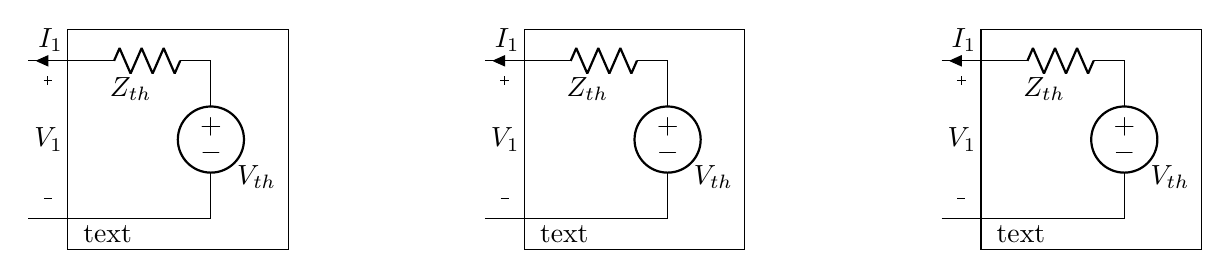
\begin{tikzpicture}
      \draw (0,0) node[Thevenin](Qa){text};
      \pingeoanchors{Qa}
      \draw (Qa.east) ++(2,0) node[Thevenin,anchor=west](Qb){text};
      \pinblackboxanchors{Qb}
      \draw (Qb.east) ++(2,0) node[Thevenin,anchor=west](Qc){text};
      \pinquadtextanchors{Qc}
    \end{tikzpicture}
  }
\end{center}



\subsubsection{Thevenin keys}
\begin{describelist*}[30mm]{keys}
  \describe {name}  {\tsmeta{node-name}, when using a to[\,] path.}
  \describe{I1}{Initial value:\tsverb{$I_1$}}
  \describe{V1}{Initial value:\tsverb{$V_1$}}
  \describe{Zth}{Initial value:\tsverb{$Z_{th}$}}
  \describe{Vth}{Initial value:\tsverb{$V_{th}$}}
  \describe{Zth label pos}{changes the label position. Defaults to: \tsobj[verb]{{south west}{top left}}}
  \describe{Vth label pos}{changes the label position. Defaults to: \tsobj[verb]{{south east}{top left}}} 
\end{describelist*}
\begin{tsremark}
The label pos keys expects two anchor names (... label pos=\tsargs[marg]{anchor A,anchor B}). The first anchors refers the sub-shape node and the second anchor is the text one.
\end{tsremark}

\subsection{Norton}
\begin{codestore}[NortonDef]
% Node use
node[Norton]{}

% To path use
(A) to[ToNorton]  (B)
\end{codestore}

\tscode*[emph={draw,node},emph2={x,y,fit,to,outer,inner,node},emph3={Quad,ToQuad,Black,ToBlack,Box,Thevenin,ToThevenin,Norton,ToNorton},basicstyle={\scriptsize\ttfamily},numbers=left,codeprefix={}]{NortonDef}
This is the classical Norton circuit. Besides the base anchors (see \ref{BBanchors}) it has 2 internal nodes: \tsobj[key]{<node>-Yn,<node>-In}  and each of those sub-nodes has geographic anchors as defined at \ref{auxiliarynodes}.
\begin{tsremark}
There is also a \tsobj[key]{ToNorton} to be used in a \tsobj[key]{to[ ]} path, in which case the key \tsobj[key]{y fit to} style will be triggered with the starting and ending points of the \tsobj[key]{to[ ]} path.
\end{tsremark}

\begin{center}%
  \resizebox{0.8\textwidth}{!}{%
    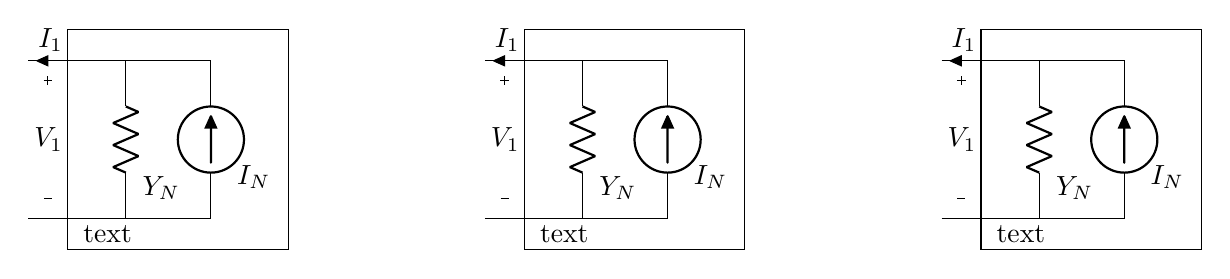
\begin{tikzpicture}
      \draw (0,0) node[Norton](Qa){text};
      \pingeoanchors{Qa}
      \draw (Qa.east) ++(2,0) node[Norton,anchor=west](Qb){text};
      \pinblackboxanchors{Qb}
      \draw (Qb.east) ++(2,0) node[Norton,anchor=west](Qc){text};
      \pinquadtextanchors{Qc}
    \end{tikzpicture}
  }
\end{center}

\subsubsection{Norton keys}
\begin{describelist*}[30mm]{keys}
  \describe {name}  {\tsmeta{node-name}, when using a to[\,] path.}
  \describe{I1}{Initial value:\tsverb{$I_1$}}
  \describe{V1}{Initial value:\tsverb{$V_1$}}
  \describe{Yn}{Initial value:\tsverb{$Y_{N}$}}
  \describe{In}{Initial value:\tsverb{$I_{N}$}}
  \describe{Yn label pos}{changes the label position. Defaults to: \tsobj[verb]{{south west}{top left}}}
  \describe{In label pos}{changes the label position. Defaults to: \tsobj[verb]{{south east}{top left}}}
\end{describelist*}
\begin{tsremark}
The label pos keys expects two anchor names (... label pos=\tsargs[marg]{anchor A,anchor B}). The first anchors refers the sub-shape node and the second anchor is the text one.
\end{tsremark}


\section{Pseudo-Graph Shape}
\begin{codestore}[PGDef]
% Node use
node[PG load line]{}

node[PG linear load line]
\end{codestore}

\tscode*[emph={draw,node},emph2={x,y,fit,to,outer,inner,node},emph3={Quad,ToQuad,Black,ToBlack,Box,Thevenin,ToThevenin,Norton,ToNorton,PG,load,line,linear},basicstyle={\scriptsize\ttfamily},numbers=left,codeprefix={}]{PGDef}

Sometimes when representing a single port sub-circuit, one might use a X-Y graph, for which \tsobj[pkg]{gnuplot,pgfplots} are excellent choices, but a bit overkill if all you want is a crude representation of a linear load line.

This shape is just that, a X-Y graph mockup, that nicely fits inside a black box, and nothing else.

\begin{center}%
%  \resizebox{0.2\textwidth}{!}{%
    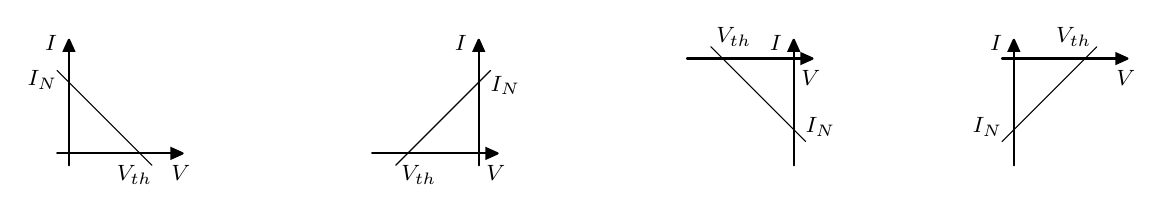
\begin{tikzpicture}
      \draw (0,0) node[PG linear load line,first quadrant](PGa){};
      \pingeoanchors{PGa}
      \draw (4,0) node[PG linear load line,second quadrant](PGa){};
      \pingeoanchors{PGa}
      \draw (8,0) node[PG linear load line,third quadrant](PGa){};
      \pingeoanchors{PGa}
      \draw (12,0) node[PG linear load line,fourth quadrant](PGa){};
      \pingeoanchors{PGa}
    \end{tikzpicture}
%  }
\end{center}


\subsection{Pseudo-Graph Keys}

These are the keys to fine tuning a shape:
\begin{describelist*}[30mm]{keys}
  \describe {x axis}  {X axis \emph{name}. Initial value: $V$}
  \describe {x val}  {X axis \emph{val} at the crossing point. Initial value: $V_{th}$}
  \describe {y axis} {Y axis \emph{name}. Initial value: $I$}
  \describe {y val} {Y axis \emph{val} at the crossing point. Initial value: $I_{N}$}
  \describe {first quadrant} {First quadrant mock up. (which is also the default).}
  \describe {second quadrant}  {Second quadrant mock up.}
  \describe {third quadrant}   {Third quadrant mock up.}
  \describe {fourth quadrant}  {Fourth quadrant mock up.}
  \describe {base width}  {The \emph{graph} width}
  \describe {half base width}  {Ditto, half width. Initial value:\tsobj{0.5\pgf@circ@Rlen}.}
  \describe {base height}  {The \emph{graph} height}
  \describe {half base height}  {Ditto, half height. Initial value:\tsobj{0.5\pgf@circ@Rlen}.}
\end{describelist*}
\begin{tsremark}
Besides these, one can also use the keys presented at \ref{generalkeys}.
\end{tsremark}


\section{Examples of use}

First of, a simple case of combining a generic Quad with equations and a generic Black Box with a Pseudo-Graph:

\begin{codestore}[DemoX]
\resizebox{\textwidth}{!}{
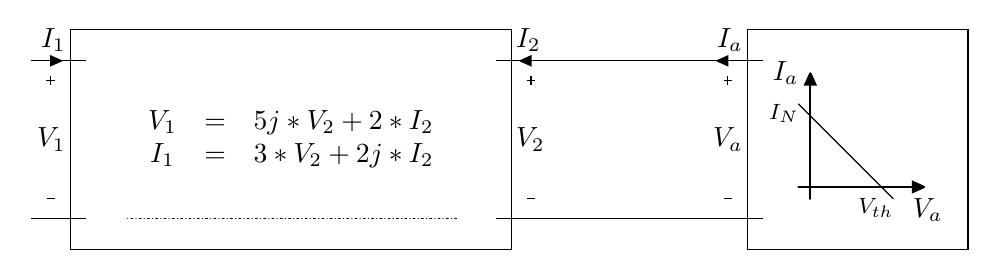
\begin{tikzpicture}
  \draw (0,0) \ncoord(ref) node[Quad,anchor=1+](Q1){}
    (Q1.2+) -- ++(1,0) \ncoord(X) -- ++(1,0) node[Black Box,anchor=1+,V1=$V_a$,I1=$I_a$](B1){}
    (Q1.2-) -- (B1.1-)
    (B1.center) node[PG linear load line,x axis=$V_a$,y axis=$I_a$]{}
    (Q1.center) node{$ \begin{matrix}
          V_1 &=& 5j*V_2 + 2*I_2 \\
          I_1 &=& 3*V_2 + 2j*I_2
        \end{matrix} $%
    }  ;
\end{tikzpicture}
}
\end{codestore}

\tsdemo*[codeprefix={},resultprefix={},emph={draw,node,coord},emph2={x,y,axis,fit,to,outer,inner,round,control,sources,european,alt},emph3={Quad,Black,Box,PG,linear,load,line},basicstyle={\scriptsize\ttfamily},numbers=left]{DemoX}

~

All default Quadripoles and Thevenin/Norton.

\begin{codestore}[DemoA]
\resizebox{\textwidth}{!}{
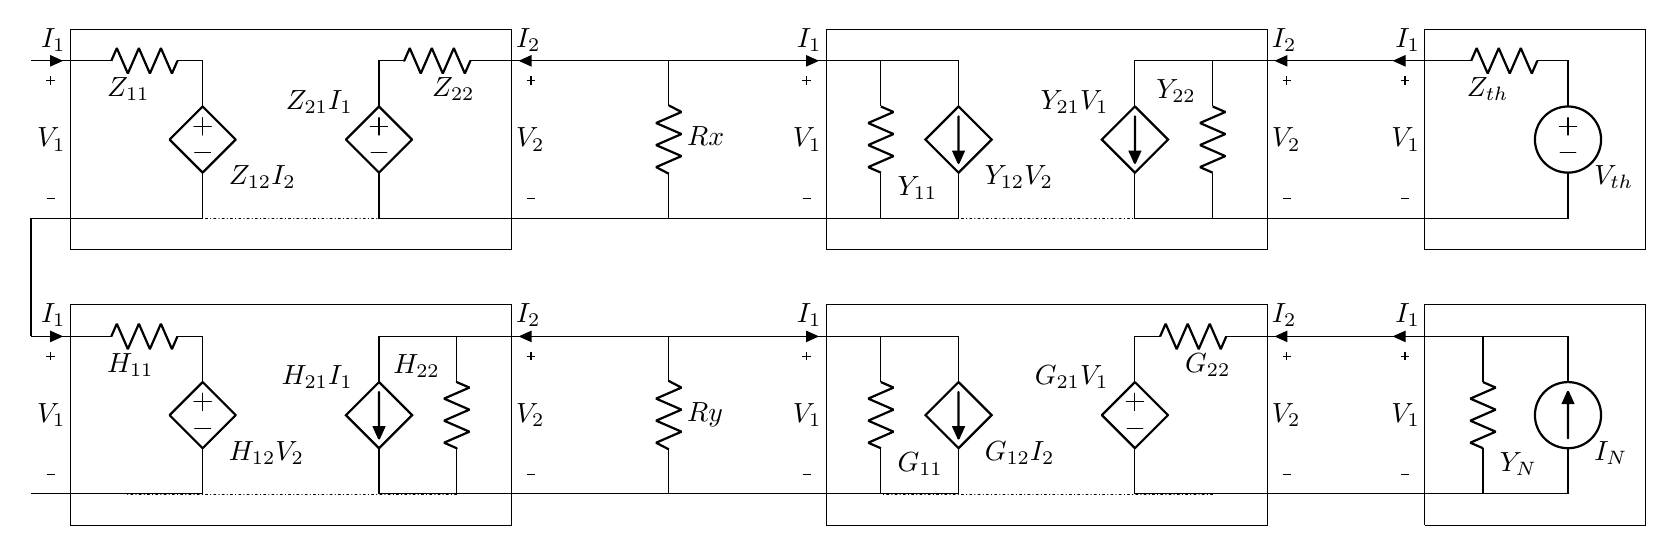
\begin{tikzpicture}
  \draw (0,0) \ncoord(ref) node[Quad Z,anchor=1+](Qz1){}
    (Qz1.2+) -- ++(1.5,0) \ncoord(X) -- ++(1.5,0) node[Quad Y,anchor=1+](Qy1){}
    (Qy1.2+) -- ++(1,0) node[Thevenin,anchor=1+](th1){}
    (Qz1.1-) -- ++(0,-1.5) node[Quad H,anchor=1+](Qh1){}
    (Qh1.2+) -- ++(1.5,0) \ncoord(Y) -- ++(1.5,0) node[Quad G,anchor=1+](Qg1){}
    (Qg1.2+) -- ++(1,0) node[Norton,anchor=1+](nr1){}
    (Qz1.2-) -- (Qy1.1-) (Qy1.2-) -- (th1.1-)
    (Qh1.2-) -- (Qg1.1-) (Qg1.2-) -- (nr1.1-)
    ;
  \draw (X) to[R=$Rx$] (X |- Qz1.2-)
        (Y) to[R=$Ry$] (Y |- Qh1.2-) 
        ;
\end{tikzpicture}
}
\end{codestore}

\tsdemo*[codeprefix={},resultprefix={},emph={draw,node,coord},emph2={x,y,fit,to,outer,inner,round,control,sources,european,alt},emph3={Quad,Black,Box},basicstyle={\scriptsize\ttfamily},numbers=left]{DemoA}

~


The same demo but with all parameter $11$ and $22$ zeroed, and changing the ``control sources''

\begin{codestore}[DemoB]
\resizebox{\textwidth}{!}{
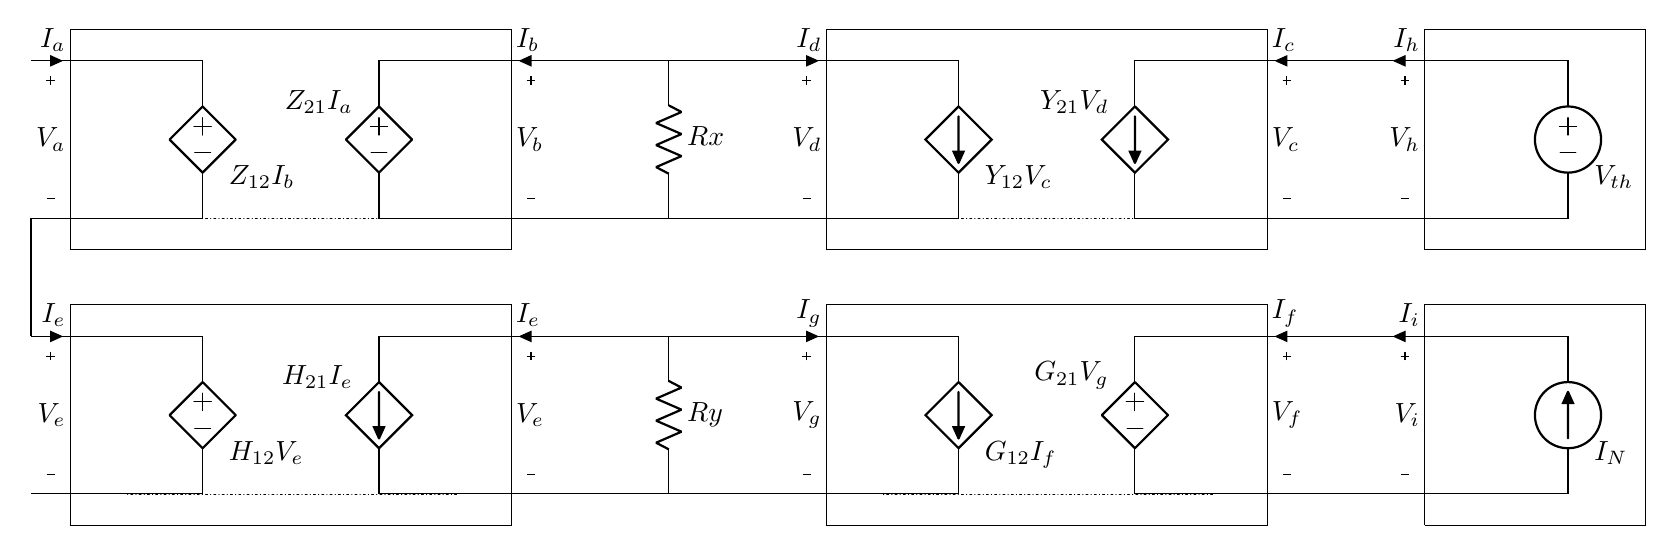
\begin{tikzpicture}
  \draw (0,0) \ncoord(ref) node[Quad Z,anchor=1+,Z11=0,Z22=0,I1=$I_a$,V1=$V_a$,I2=$I_b$,V2=$V_b$](Qz1){}
    (Qz1.2+) -- ++(1.5,0) \ncoord(X) -- ++(1.5,0) node[Quad Y,anchor=1+,Y11=0,Y22=0,I1=$I_d$,V1=$V_d$,I2=$I_c$,V2=$V_c$](Qy1){}
    (Qy1.2+) -- ++(1,0) node[Thevenin,anchor=1+,Zth=0,I1=$I_h$,V1=$V_h$](th1){}
    (Qz1.1-) -- ++(0,-1.5) node[Quad H,anchor=1+,H11=0,H22=0,I1=$I_e$,V1=$V_e$,I2=$I_e$,V2=$V_e$](Qh1){}
    (Qh1.2+) -- ++(1.5,0) \ncoord(Y) -- ++(1.5,0) node[Quad G,anchor=1+,G11=0,G22=0,I1=$I_g$,V1=$V_g$,I2=$I_f$,V2=$V_f$](Qg1){}
    (Qg1.2+) -- ++(1,0) node[Norton,anchor=1+,Yn=0,I1=$I_i$,V1=$V_i$](nr1){}
    (Qz1.2-) -- (Qy1.1-) (Qy1.2-) -- (th1.1-)
    (Qh1.2-) -- (Qg1.1-) (Qg1.2-) -- (nr1.1-)
    ;
  \draw (X) to[R=$Rx$] (X |- Qz1.2-)
        (Y) to[R=$Ry$] (Y |- Qh1.2-) 
        ;
\end{tikzpicture}
}
\end{codestore}

\tsdemo*[codeprefix={},resultprefix={},emph={draw,node,coord},emph2={x,y,fit,to,outer,inner,round,control,sources,european,alt},emph3={Quad,Black,Box},basicstyle={\scriptsize\ttfamily},numbers=left]{DemoB}
~


Now with the $12$ and $21$ parameters zeroed, normal form:

\begin{codestore}[DemoC]
\resizebox{\textwidth}{!}{
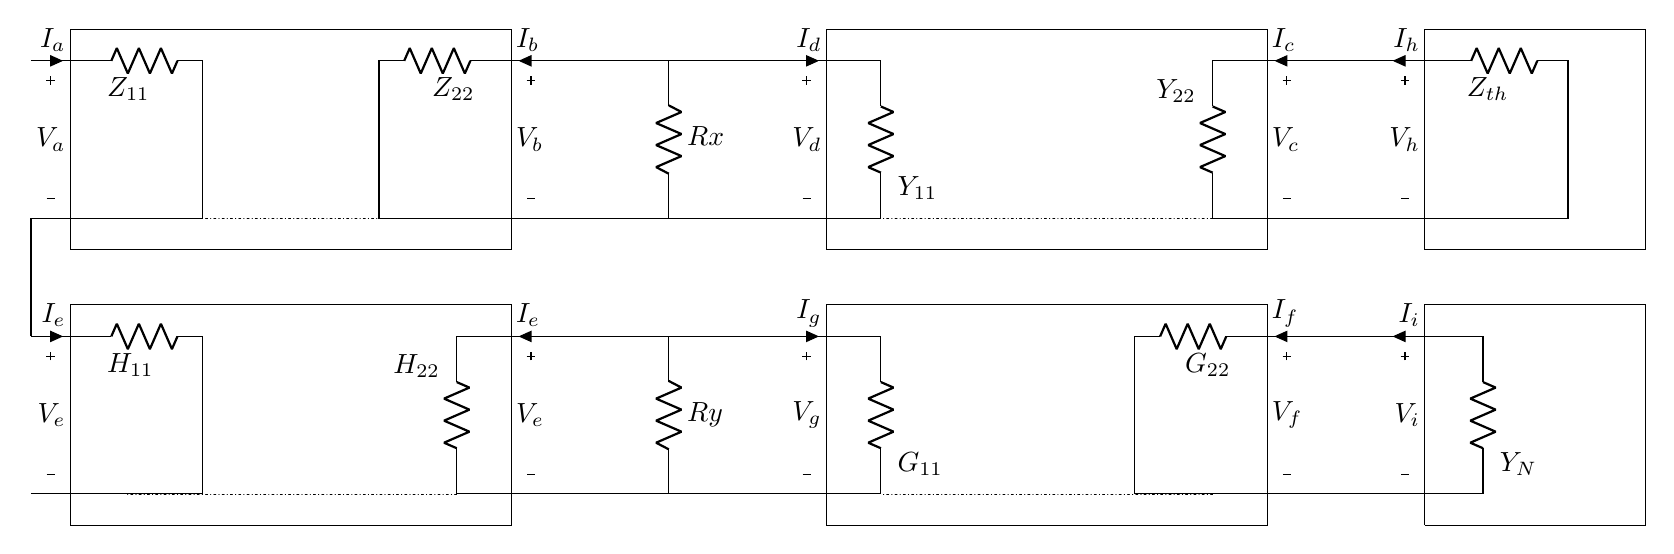
\begin{tikzpicture}
  \draw (0,0) \ncoord(ref) node[Quad Z,anchor=1+,Z12=0,Z21=0,I1=$I_a$,V1=$V_a$,I2=$I_b$,V2=$V_b$](Qz1){}
    (Qz1.2+) -- ++(1.5,0) \ncoord(X) -- ++(1.5,0) node[Quad Y,anchor=1+,Y12=0,Y21=0,I1=$I_d$,V1=$V_d$,I2=$I_c$,V2=$V_c$](Qy1){}
    (Qy1.2+) -- ++(1,0) node[Thevenin,anchor=1+,Vth=0,I1=$I_h$,V1=$V_h$](th1){}
    (Qz1.1-) -- ++(0,-1.5) node[Quad H,anchor=1+,H12=0,H21=0,I1=$I_e$,V1=$V_e$,I2=$I_e$,V2=$V_e$](Qh1){}
    (Qh1.2+) -- ++(1.5,0) \ncoord(Y) -- ++(1.5,0) node[Quad G,anchor=1+,G12=0,G21=0,I1=$I_g$,V1=$V_g$,I2=$I_f$,V2=$V_f$](Qg1){}
    (Qg1.2+) -- ++(1,0) node[Norton,anchor=1+,In=0,I1=$I_i$,V1=$V_i$](nr1){}
    (Qz1.2-) -- (Qy1.1-) (Qy1.2-) -- (th1.1-)
    (Qh1.2-) -- (Qg1.1-) (Qg1.2-) -- (nr1.1-)
    ;
  \draw (X) to[R=$Rx$] (X |- Qz1.2-)
        (Y) to[R=$Ry$] (Y |- Qh1.2-) 
        ;
\end{tikzpicture}
}
\end{codestore}

\tsdemo*[codeprefix={},resultprefix={},emph={draw,node,coord},emph2={x,y,fit,to,outer,inner,round,control,sources,european,alt},emph3={Quad,Black,Box},basicstyle={\scriptsize\ttfamily},numbers=left]{DemoC}

~

Same as last one, but with an alternate form:

\begin{codestore}[DemoC]
\resizebox{\textwidth}{!}{
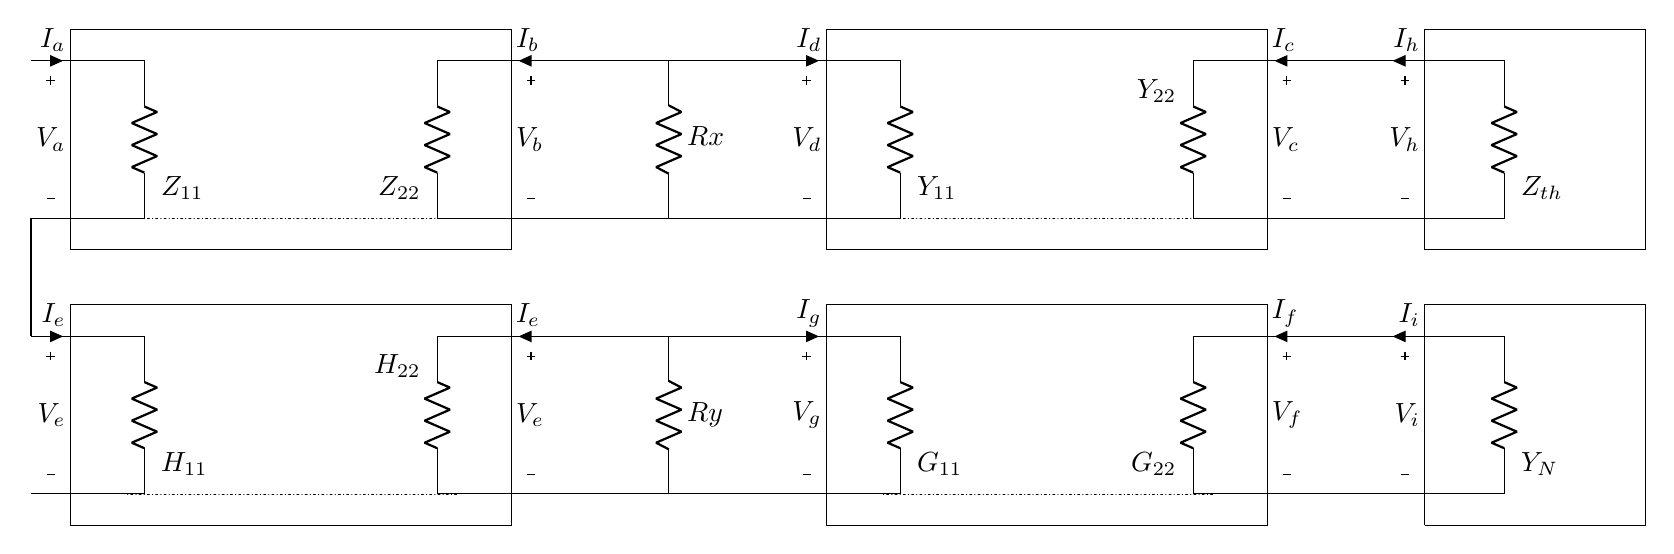
\begin{tikzpicture}
  \draw (0,0) \ncoord(ref) node[Quad Z,alt,anchor=1+,Z12=0,Z21=0,I1=$I_a$,V1=$V_a$,I2=$I_b$,V2=$V_b$](Qz1){}
    (Qz1.2+) -- ++(1.5,0) \ncoord(X) -- ++(1.5,0) node[Quad Y,alt,anchor=1+,Y12=0,Y21=0,I1=$I_d$,V1=$V_d$,I2=$I_c$,V2=$V_c$](Qy1){}
    (Qy1.2+) -- ++(1,0) node[Thevenin,alt,anchor=1+,Vth=0,I1=$I_h$,V1=$V_h$](th1){}
    (Qz1.1-) -- ++(0,-1.5) node[Quad H,alt,anchor=1+,H12=0,H21=0,I1=$I_e$,V1=$V_e$,I2=$I_e$,V2=$V_e$](Qh1){}
    (Qh1.2+) -- ++(1.5,0) \ncoord(Y) -- ++(1.5,0) node[Quad G,alt,anchor=1+,G12=0,G21=0,I1=$I_g$,V1=$V_g$,I2=$I_f$,V2=$V_f$](Qg1){}
    (Qg1.2+) -- ++(1,0) node[Norton,alt,anchor=1+,In=0,I1=$I_i$,V1=$V_i$](nr1){}
    (Qz1.2-) -- (Qy1.1-) (Qy1.2-) -- (th1.1-)
    (Qh1.2-) -- (Qg1.1-) (Qg1.2-) -- (nr1.1-)
    ;
  \draw (X) to[R=$Rx$] (X |- Qz1.2-)
        (Y) to[R=$Ry$] (Y |- Qh1.2-) 
        ;
\end{tikzpicture}
}
\end{codestore}

\tsdemo*[codeprefix={},resultprefix={},emph={draw,node,coord},emph2={x,y,fit,to,outer,inner,round,control,sources,european,alt},emph3={Quad,Black,Box},basicstyle={\scriptsize\ttfamily},numbers=left]{DemoC}

~


Setting all parameters,some impedances as zig-zag, others as generic, per quadripole:



\begin{codestore}[DemoD]
\resizebox{\textwidth}{!}{
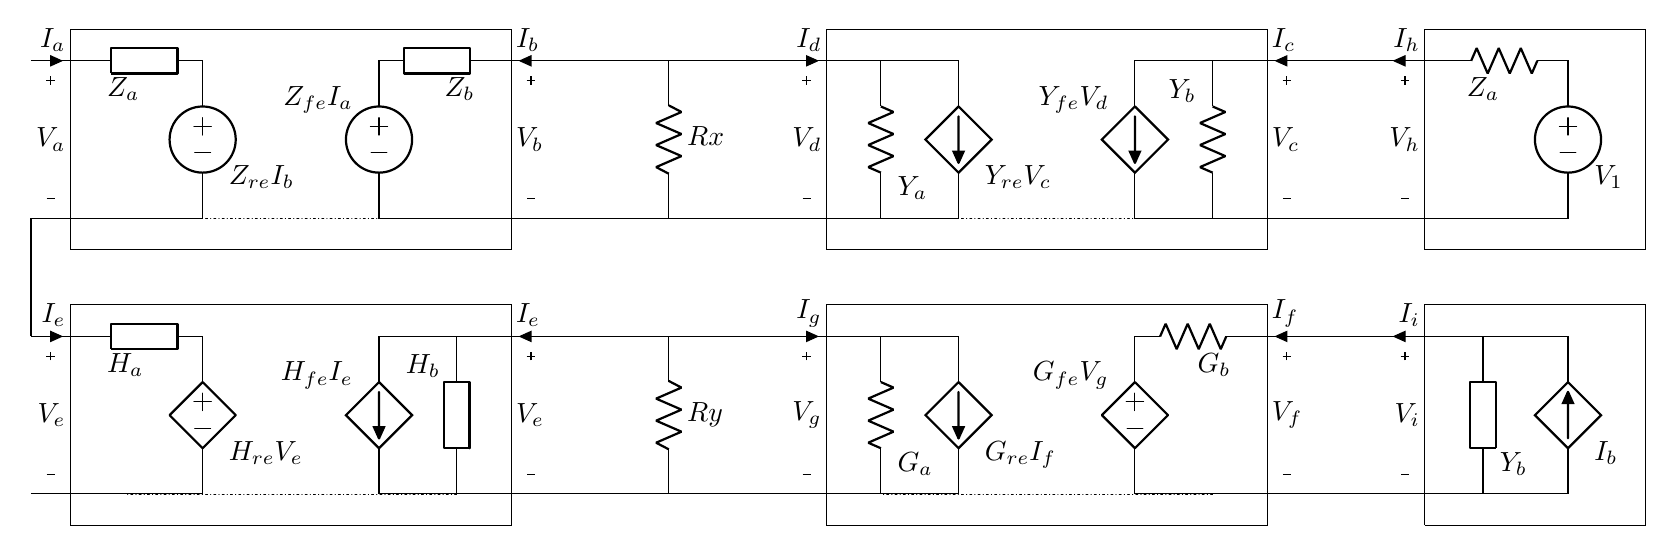
\begin{tikzpicture}
  \draw (0,0) \ncoord(ref) node[Quad Z,alt,round sources,european,anchor=1+,Z11=$Z_a$,Z22=$Z_b$,Z12=$Z_{re}$,Z21=$Z_{fe}$,I1=$I_a$,V1=$V_a$,I2=$I_b$,V2=$V_b$](Qz1){}
    (Qz1.2+) -- ++(1.5,0) \ncoord(X) -- ++(1.5,0) node[Quad Y,alt,anchor=1+,Y11=$Y_a$,Y22=$Y_b$,Y12=$Y_{re}$,Y21=$Y_{fe}$,I1=$I_d$,V1=$V_d$,I2=$I_c$,V2=$V_c$](Qy1){}
    (Qy1.2+) -- ++(1,0) node[Thevenin,alt,anchor=1+,Vth=$V_1$,Zth=$Z_a$,I1=$I_h$,V1=$V_h$](th1){}
    (Qz1.1-) -- ++(0,-1.5) node[Quad H,european,alt,anchor=1+,H11=$H_a$,H22=$H_b$,H12=$H_{re}$,H21=$H_{fe}$,I1=$I_e$,V1=$V_e$,I2=$I_e$,V2=$V_e$](Qh1){}
    (Qh1.2+) -- ++(1.5,0) \ncoord(Y) -- ++(1.5,0) node[Quad G,alt,anchor=1+,G11=$G_a$,G22=$G_b$,G12=$G_{re}$,G21=$G_{fe}$,I1=$I_g$,V1=$V_g$,I2=$I_f$,V2=$V_f$](Qg1){}
    (Qg1.2+) -- ++(1,0) node[Norton,alt,control sources,european,anchor=1+,In=$I_b$,Yn=$Y_b$,I1=$I_i$,V1=$V_i$](nr1){}
    (Qz1.2-) -- (Qy1.1-) (Qy1.2-) -- (th1.1-)
    (Qh1.2-) -- (Qg1.1-) (Qg1.2-) -- (nr1.1-)
    ;
  \draw (X) to[R=$Rx$] (X |- Qz1.2-)
        (Y) to[R=$Ry$] (Y |- Qh1.2-) 
        ;
\end{tikzpicture}
}
\end{codestore}

\tsdemo*[codeprefix={},resultprefix={},emph={draw,node,coord},emph2={x,y,fit,to,outer,inner,round,control,sources,european,alt},emph3={Quad,Black,Box},basicstyle={\scriptsize\ttfamily},numbers=left]{DemoD}



\end{document}
